\chapter{Threshold Moore}
\label{chap:tm}

\section{Theory}

\begin{defn}
	Let $\mathcal{A} = (Q, \Sigma, \delta, c)$ be a DPA. For a set $K \subseteq \mathbb{N}$, we define the \emph{priority threshold} of $\mathcal{A}$ as $\mathcal{T}(\mathcal{A}, >k) := (Q, \Sigma, \delta, c')$ with $c'(q) = \begin{cases} c(q) & \text{if } c(q) \leq k \\ k + 1 & \text{else} \end{cases}$.
	
	For a relation $\sim$, we define $\mathcal{T}(\sim, >k) :=\, \approx$ as $(\mathcal{A}, p) \approx (\mathcal{B}, q)$ iff $(\mathcal{T}(\mathcal{A}, >k), p) \sim (\mathcal{T}(\mathcal{B}, >k), q)$.
\end{defn}

\begin{lem}
	If $\sim$ is an equivalence relation, then so is $\mathcal{T}(\sim, >k)$. If $\sim$ is a congruence relation, then so is $\mathcal{T}(\sim, >k)$.
\end{lem}

\begin{proof}
	This follows directly by plugging in definitions. For example, assume that $\approx \,= \mathcal{T}(\sim, >k)$ is not symmetric, so $(\mathcal{A}, p) \approx (\mathcal{B}, q)$ but $(\mathcal{B}, q) \not\approx (\mathcal{A}, p)$. Then $(\mathcal{T}(\mathcal{A}, >k), p) \sim (\mathcal{T}(\mathcal{B}, >k), q)$ but $(\mathcal{T}(\mathcal{B}, >k), q) \not\sim (\mathcal{T}(\mathcal{A}, >k), p)$ and thus $\sim$ is not symmetric either.
\end{proof}

\begin{defn}
	We set $\equiv_M^{\leq k} \,:= \mathcal{T}(\equiv_M, >k)$.
\end{defn}

\begin{lem}
	For two numbers $x, y \in \mathbb{N}$, let $x =^{\leq k} y$ iff $x = y$ or $\min \{x, y\} > k$. Then $(\mathcal{A}, p) \equiv_M^{\leq k} (\mathcal{B}, q)$ iff for all $w \in \Sigma^*$, $c_1(\delta_1^*(p, w)) =^{\leq k} c_2(\delta_2^*(q, w))$.
\end{lem}

\begin{proof}
	$(\mathcal{A}, p) \equiv_M^{\leq k} (\mathcal{B}, q)$ is true iff $(\mathcal{T}(\mathcal{A}, >k), p) \equiv_M (\mathcal{T}(\mathcal{B}, >k), q)$ iff for all $w \in \Sigma^*$, $c'_1(\delta_1^*(p, w)) = c'_2(\delta_2^*(q, w)$. If we compare definitions, it becomes clear that $c'_1(x) = c'_2(y)$ iff $c_1(x) =^{\leq k} c_2(y)$.
\end{proof}

\vspace{5pt}

\begin{defn}
	Let $\mathcal{A}$ and $\mathcal{B}$ be DPAs and let $\sim$ be an equivalence relation that implies language equivalence. We define a relation $\equiv_\text{TM}^\sim$ such that $(\mathcal{A}, p) \equiv^\sim_\text{TM} (\mathcal{B}, q)$ if and only if all of the following are satisfied:
	\begin{enumerate}
		\item $c_1(p) = c_2(q)$
		\item $(\mathcal{A}, p) \equiv_M^{\leq c(p)} (\mathcal{B}, q)$
		\item $(\mathcal{A}, p) \sim (\mathcal{B}, q)$
	\end{enumerate}
\end{defn}

\vspace{5pt}

We can notice that merging classes of $\equiv_\text{TM}^\sim$ in a specific order is a valid language-preserving operation. This is then used to define a fitting merger function. For this next part, let $\mathcal{A}$ be a DPA and let $\kappa \in \mathfrak{C}(\equiv^\sim_\text{TM})$ be a set of states in $\mathcal{A}$. By definition of $\equiv^\sim_\text{TM}$, all states in this class have a unique priority $k$. Let $\mathcal{A}'$ be a representative merge of $\mathcal{A}$ w.r.t. $\kappa$.

\begin{lem}
	For all $q \in Q'$, $(\mathcal{A}, q) \equiv_L (\mathcal{A}', q)$.
	\label{lem:tremoore:merge_keep_lang}
\end{lem}

\begin{proof} 
	Let $\rho$ and $\rho'$ be the runs of $\mathcal{A}$ and $\mathcal{A}'$ on some $\alpha \in \Sigma^\omega$ starting from $q$. We claim that $\rho$ is accepting iff $\rho'$ is accepting.
	
	By Lemma \ref{lem:general:cong_stays_in_merge}, $(\mathcal{A}, \rho(i)) \equiv_L (\mathcal{A}, \rho'(i))$ and $(\mathcal{A}, \rho(i)) \equiv_M^{\leq k} (\mathcal{A}, \rho'(i))$ for all $i$. Now there are two cases: if $c(\rho)$ sees infinitely many priorities of at most $k$, then $c(\rho')$ sees the same priorities at the same positions and thus $\min \text{Inf}(c(\rho)) = \min \text{Inf}(c(\rho'))$. By definition of a representative merge, $c(\rho') = c'(\rho')$.
	
	 Otherwise there is a position $n$ from which $c(\rho)$ only is greater than $k$ and therefore the same is true for $c(\rho')$. That means reading $\alpha[n,\omega]$ from $\rho'(n)$ in either $\mathcal{A}$ or $\mathcal{A}'$ yields the same run which has the same acceptance as $\rho$.
\end{proof}

\vspace{10pt}

The research becomes more interesting if you fix $\sim$ to be the complete language equivalence $\equiv_L$, which is what we consider for the next Lemmas.

\begin{lem}
	For all $q \in Q'$ with $c(q) \leq k$, $(\mathcal{A}, q) \equiv_M^{\leq k} (\mathcal{A}', q)$.
	\label{lem:tremoore:merge_keep_tmoore}
\end{lem}

\begin{proof} 
	Let $\rho$ and $\rho'$ be the runs of $\mathcal{A}$ and $\mathcal{A}'$ on $\alpha \in \Sigma^\omega$ starting from $q$. We claim that $c(\rho(i)) =^{\leq k} c'(\rho'(i))$ for all $i$ which then proves the Lemma.
	
	By Lemma \ref{lem:general:cong_stays_in_merge}, $(\mathcal{A}, \rho(i)) \equiv_M^{\leq k} (\mathcal{A}, \rho'(i))$ for all $i$ which especially means that for all $i$, $c(\rho(i)) =^{\leq k} c(\rho'(i))$. Since $c(\rho'(i)) = c'(\rho'(i))$, that also implies $c(\rho(i)) =^{\leq k} c'(\rho'(i))$.
\end{proof}

\begin{lem}
	Let $l \leq k \in \mathbb{N}$. Then $\equiv_M^{\leq k} \,\subseteq\, \equiv_M^{\leq l}$.
	\label{lem:tremoore:moore_less_thresh_is_subset}
\end{lem}

\begin{proof}
	Let $\mathcal{A} = (Q_1, \Sigma, \delta_1, c_1)$ and $\mathcal{B} = (Q_2, \Sigma, \delta_2, c_2)$ be two DPAs. Let $\mathcal{A}^{\leq l} = \mathcal{T}(\mathcal{A}, > l)$ and $\mathcal{A}^{\leq k}$, $\mathcal{B}^{\leq l}$, and $\mathcal{B}^{\leq k}$ analogously.
	
	Let $(\mathcal{A}, p) \not\equiv_M^{\leq l} (\mathcal{B}, q)$, so there is a word $w \in \Sigma^*$ such that $c_1^{\leq l}(p') \neq c_2^{\leq l}(q')$, where $p' = \delta_1^*(p, w)$ and $q' = \delta_2^*(q, w)$. This means at least one of $c_1(p')$ and $c_2(q')$ is at most $l$, as otherwise both these values would be set to $l+1$. Due to symmetry, we can assume that $c_1(p')$ is that value.
	
	As $l \leq k$, $c_1^{\leq k}(p') = c_1^{\leq l}(p')$ and $c_2^{\leq k}(q') \geq c_2^{\leq l}(q')$, so $c_1^{\leq k}(p') \neq c_2^{\leq k}(q')$ and thus $(\mathcal{A}, p) \not\equiv_M^{\leq k} (\mathcal{B}, q)$.
\end{proof} 

\begin{lem}
	For all $q \in Q'$ with $c(q) \leq k$, $(\mathcal{A}, q) \equiv^{\equiv_L}_\text{TM} (\mathcal{A}', q)$.
	\label{lem:tremoore:merge_keep_tm}
\end{lem}

\begin{proof}
	Representative merges never change priorities assigned to states. Together with Lemma \ref{lem:tremoore:merge_keep_lang}, Lemma \ref{lem:tremoore:merge_keep_tmoore}, and Lemma \ref{lem:tremoore:moore_less_thresh_is_subset} this already finishes the proof.
\end{proof}

\begin{lem}
	For all $p, q \in Q'$ with $\min \{c(p), c(q)\} \leq k$, $(\mathcal{A}, p) \equiv^{\equiv_L}_\text{TM} (\mathcal{A}, q)$ iff \linebreak $(\mathcal{A}', p) \equiv^{\equiv_L}_\text{TM} (\mathcal{A}', q)$.
	\label{lem:tremoore:merge_changes_only_higher}
\end{lem}

\begin{proof}
	If $c(p) = c(q) \leq k$: By Lemma \ref{lem:tremoore:merge_keep_tm}, we know that $(\mathcal{A}, p) \equiv^{\equiv_L}_\text{TM} (\mathcal{A}', p)$ and $(\mathcal{A}, q) \equiv^{\equiv_L}_\text{TM} (\mathcal{A}', q)$. If now $(\mathcal{A}, p) \equiv^{\equiv_L}_\text{TM} (\mathcal{A}, q)$ holds, then also $(\mathcal{A}', p) \equiv^{\equiv_L}_\text{TM} (\mathcal{A}', q)$ and vice versa.
	
	If $c(p) \neq c(q)$, then also $c'(p) \neq c'(q)$ and we have both $(\mathcal{A}, p) \not\equiv^{\equiv_L}_\text{TM} (\mathcal{A}, q)$ and $(\mathcal{A}', p) \not\equiv^{\equiv_L}_\text{TM} (\mathcal{A}', q)$.
\end{proof}

\vspace{10pt}

\begin{defn}
	Let $\mathcal{A}$ be a DPA and let $\sim$ be an equivalence relation that implies language equivalence. We define the \emph{Threshold Moore merger function} $\mu_\text{TM}^\sim := \mu_\div^{\equiv^\sim_\text{TM}}$.
\end{defn}

\begin{theorem}
	Every representative merge of a DPA $\mathcal{A}$ w.r.t. $\mu_\text{TM}^{\equiv_L}$ is language equivalent to $\mathcal{A}$.
\end{theorem}

\begin{proof}
	Building a representative merge of $\mathcal{A}$ w.r.t. $\mu_\text{TM}^{\equiv_L}$ implicitly builds multiple representative merges $\mathcal{A}_0, \dots, \mathcal{A}_m$, where $\mathcal{A}_{i+1}$ is a representative merge of $\mathcal{A}_i$ w.r.t. some $\kappa_i$. By Lemma \ref{lem:tremoore:merge_changes_only_higher}, for all $j > i$, the states in $\kappa_j$ are still pairwise $\equiv^{\equiv_L}_\text{TM}$ equivalent. Moreover, $\kappa_{i+1}$ is an $\equiv^{\equiv_L}_\text{TM}$ equivalence class in $\mathcal{A}_i$. That means we can continue building representative merges in order of the enumeration and our previous results apply. In the end, we obtain a DPA $\mathcal{A}'$ that is language equivalent to $\mathcal{A}$ by Lemma \ref{lem:tremoore:merge_keep_lang}.
\end{proof}

\section{Computation}
\begin{lem}
	For a given DPA, $\equiv_M^{\leq k}$ can be computed in $\mathcal{O}(|Q| \cdot \log |Q|)$.
	\label{lem:tremoore:kmoore_loglin}
\end{lem}

\begin{proof}
	Computing $\mathcal{T}(\mathcal{A}, >k)$ can clearly be done in linear time. The rest follows from Corollary \ref{cor:general:M_loglin}.
\end{proof}

\begin{lem}
	For a given $\mathcal{A}$ and equivalence relation $\sim$, $\mu_\text{TM}^\sim$ can be computed in $\mathcal{O}(|Q| \cdot \log |Q| \cdot |c(Q)|)$.
\end{lem}

\begin{proof}
	First, we compute $\equiv_M^{\leq k}$ for all $k \in c(Q)$. This can be done in $\mathcal{O}(|Q| \cdot \log |Q| \cdot |c(Q)|)$ by Lemma \ref{lem:tremoore:kmoore_loglin}. After that, we build the restriction of $\equiv_M^{\leq k}$ to $c^{-1}(k)$ for every $k$ and then again find the union of all those sets. Both steps can be done in linear time. Finally, the result of this operation has to be intersected with $\sim$ which is also possible in linear time given a suitable data structure for $\sim$. This then gives us $\equiv_\text{TM}^\sim$. As $\mu_\text{TM}^\sim$ is a simple quotient merger, there is no additional work to be done.
\end{proof}



\section{Efficiency}
Figures \ref{fig:tremoore:empirical_size_hist} and \ref{fig:tremoore:empirical_reduct_rel} show that, unfortunately, the Threshold Moore merger only has very little effect on the \textsf{gendet} and \textsf{detnbaut} data sets. Comparing the results for \textsf{detspot} to those of $\mu_M$ in figure \ref{fig:general:empirical_moore_size_hist} shows that there is not much gain here either. Even though the results of the reduction are disappointing, it still requires us to compute some kind of relation $\sim$; in our case we used $\equiv_L$ again, which also had a noticeable impact on the run time as can be seen in figure \ref{fig:tremoore:empirical_time}.

Like for the path refinement merger, we could use the internal equivalence relation of \textsf{detnbaut} to eliminate the need of explicitly calculating $\sim$. However, as we already barely achieved any reduction with $\equiv_L$ and \enquote{worse} relations only decrease the amount of reduction, this step seems obsolete.


\begin{figure}
	\centering
	\begin{minipage}{0.49\textwidth}
		\includegraphics[page=6,height=.3\textheight]{../data/analysis/threshold_moore/gendet_ap1.pdf} 
		\includegraphics[page=6,height=.3\textheight]{../data/analysis/threshold_moore/detspot_ap1.pdf} 
		\includegraphics[page=6,height=.3\textheight]{../data/analysis/threshold_moore/detnbaut_ap1.pdf} 
		\caption{State reduction of different automata using $\mu_\text{TM}^{\equiv_L}$.}
		\label{fig:tremoore:empirical_size_hist}
	\end{minipage}
	\hfill
	\begin{minipage}{0.49\textwidth}
		\includegraphics[page=3,height=.3\textheight]{../data/analysis/threshold_moore/gendet_ap1.pdf} 
		\includegraphics[page=3,height=.3\textheight]{../data/analysis/threshold_moore/detspot_ap1.pdf} 
		\includegraphics[page=3,height=.3\textheight]{../data/analysis/threshold_moore/detnbaut_ap1.pdf} 
		\caption{Relative state reduction of different automata using $\mu_\text{TM}^{\equiv_L}$.}
		\label{fig:tremoore:empirical_reduct_rel}
	\end{minipage}
\end{figure}

\begin{figure}
	\centering
	\begin{minipage}{0.49\textwidth}
		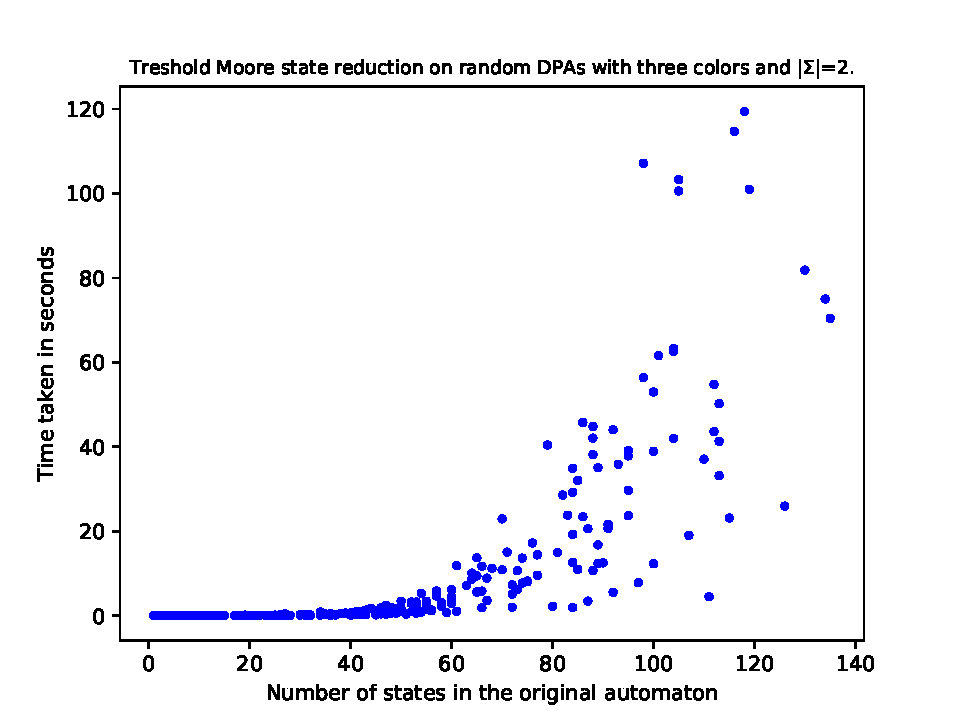
\includegraphics[page=1,height=.3\textheight]{../data/analysis/threshold_moore/gendet_ap1.pdf} 
		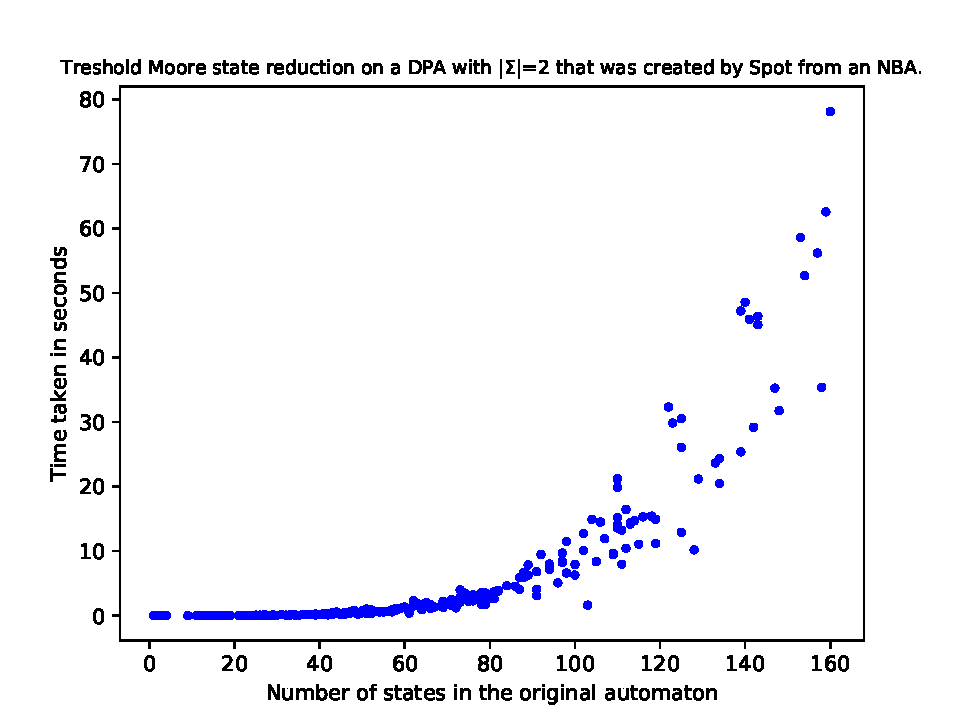
\includegraphics[page=1,height=.3\textheight]{../data/analysis/threshold_moore/detspot_ap1.pdf} 
		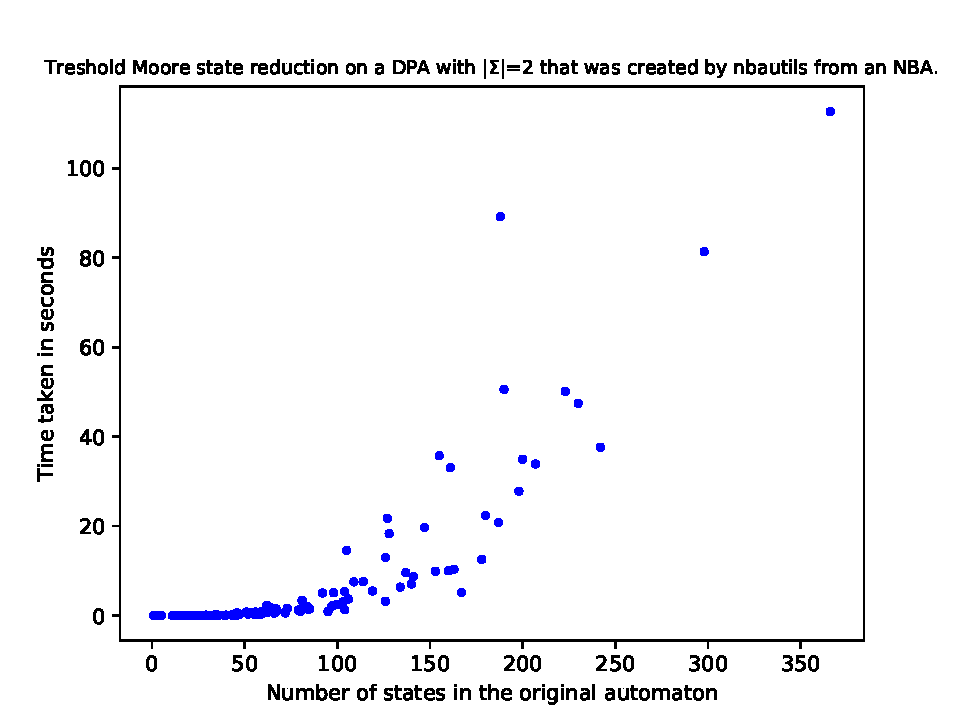
\includegraphics[page=1,height=.3\textheight]{../data/analysis/threshold_moore/detnbaut_ap1.pdf} 
		\caption{Time for state reduction of different automata using $\mu_\text{TM}^{\equiv_L}$.}
		\label{fig:tremoore:empirical_time}
	\end{minipage}
\end{figure}




\section{Different Thresholds}

An interesting question to ask ourselves is whether changing $\equiv_M$ in the definition of $\equiv_\text{TM}^\sim$ to a weaker relation still offers the same qualities, especially the language equivalence. One might especially look for a set of properties that a general equivalence relation $\sim'$ has to satisfy so that we can replace $\equiv_M$. As it turns out, this is not easy to do.

In fact, figure \ref{fig:tremoore:desim_counterex1} displays an automaton that shows that replacing $\equiv_M$ by $\equiv_\text{de}$ will not preserve language when used in a merge. For this purpose we will call this variation of $\equiv_\text{Tde}$ instead and fix $\sim \,=\, \equiv_L$ to be the complete language equivalence.

The equivalence classes are $\mathfrak{C}(\equiv_\text{Tde}) = \{ \{q_0, q_2\}, \{q_1\}, \{q_3\} \}$, which means the automaton shown in figure \ref{fig:tremoore:desim_counterex2} is a representative merge. However, this automaton rejects every word which is not the case for the original.

\begin{figure}
\centering
\begin{tikzpicture}[shorten >=1pt,node distance=2cm,on grid,initial text=]
  \node[state] (0)           	{$q_0$,\{2\}};
  \node[state] (1) [right=of 0] {$q_1$,\{1\}};
  \node[state] (2) [right=of 1] {$q_2$,\{2\}};
  \node[state] (3) [right=of 2] {$q_3$,\{0\}};
  \path[->] (0) edge node [above] {a} (1)
            (1) edge node [above] {a} (2)
            (2) edge [bend left] node [above] {a} (3)
            (3) edge [bend left] node [above] {a} (2);
\end{tikzpicture}
\caption{Example automaton which shows that using $\equiv_\text{de}$ for $\equiv_\text{TM}$ will not work.}
\label{fig:tremoore:desim_counterex1}
\end{figure}

\begin{figure}
\centering
\begin{tikzpicture}[shorten >=1pt,node distance=2cm,on grid,initial text=]
  \node[state] (1)           	{$q_1$,\{1\}};
  \node[state] (0) [right=of 1] {$q_0$,\{2\}};
  \node[state] (3) [right=of 0] {$q_3$,\{0\}};
  \path[->] (0) edge [bend left] node [above] {a} (1)
            (1) edge [bend left] node [above] {a} (0)
            (3) edge node [above] {a} (0);
\end{tikzpicture}
\caption{Example automaton which shows that using $\equiv_\text{de}$ for $\equiv_\text{TM}$ will not work.}
\label{fig:tremoore:desim_counterex2}
\end{figure}








